\documentclass[11pt,a4paper]{article}

\usepackage[utf8]{inputenc}
\usepackage[T1]{fontenc}
\usepackage{lmodern}
\usepackage[margin=1in]{geometry}
\usepackage{booktabs}
\usepackage{listings}
\usepackage{xcolor}
\usepackage{hyperref}
\usepackage{tikz}
\usepackage{enumitem}
\usepackage{amsmath}
\usepackage{fancyhdr}
\usepackage{float}
\usepackage{caption}
\usepackage{needspace}

% Prevent hyphenation inside \texttt — push to next line instead
\renewcommand{\texttt}[1]{{\ttfamily\hyphenpenalty=10000\exhyphenpenalty=10000 #1}}
% Allow extra interword stretch so non-hyphenated \texttt wraps cleanly
\emergencystretch=3em

\usetikzlibrary{arrows.meta, positioning, shapes.geometric, fit, calc,
    decorations.pathreplacing}

\hypersetup{
    colorlinks=true,
    linkcolor=blue!60!black,
    urlcolor=blue!60!black,
    citecolor=blue!60!black,
    pdftitle={Cross-Queue XDP Redirect to AF\_XDP Sockets with Shared UMEM},
    pdfauthor={Alex Dvoretsky},
}

\lstset{
    basicstyle=\ttfamily\small,
    breaklines=true,
    frame=single,
    backgroundcolor=\color{gray!8},
    keywordstyle=\color{blue!70!black}\bfseries,
    commentstyle=\color{green!50!black}\itshape,
    stringstyle=\color{red!60!black},
    numbers=left,
    numberstyle=\tiny\color{gray},
    numbersep=5pt,
    tabsize=4,
    showstringspaces=false,
    language=C,
    morekeywords={u32, u64, u16, __u32, __u64, bool, dma_addr_t,
        xdp_buff, xdp_buff_xsk, xdp_sock, xsk_buff_pool,
        bpf_redirect_map, xdp_do_redirect, SEC, __uint, __type},
}

\pagestyle{fancy}
\fancyhf{}
\fancyhead[L]{\small Cross-Queue XDP Redirect to XSK Sockets}
\fancyhead[R]{\small \thepage}
\renewcommand{\headrulewidth}{0.4pt}

\title{%
    \Large Cross-Queue \texttt{XDP\_REDIRECT} to AF\_XDP Sockets\\
    with Shared UMEM in Zero-Copy Mode\\[0.5em]
    \large Analysis of the \texttt{xsk\_rcv\_check()} Guard\\
    and Proposal for Relaxation
}
\author{Claude Code (Anthropic)\\[0.3em]
    \normalsize by request and with guidance of Alex Dvoretsky}
\date{April 2026}

\begin{document}
\maketitle

\begin{abstract}
AF\_XDP sockets bound to different hardware queues on the same NIC cannot
receive cross-queue redirected frames, even when sharing a single UMEM region.
The kernel enforces a \texttt{queue\_id} equality check in
\texttt{xsk\_rcv\_check()} (net/xdp/xsk.c) that silently drops any frame
whose receive queue index differs from the target socket's bound queue.
This paper traces the complete redirect code path---from driver NAPI handler
through the generic XSK layer---and demonstrates that for aligned shared-UMEM
configurations, the check is the \emph{sole} barrier to correct cross-queue
delivery. No driver modifications are required. We address concerns regarding
ring index management, buffer ownership transfer, DMA coherency, teardown
safety, and pool accounting, showing that each is handled correctly by
existing code. We propose a minimal kernel patch to relax the guard for
sockets sharing the same UMEM, enabling hardware-queue-level packet steering
within a single AF\_XDP application.
\end{abstract}

\tableofcontents

\section{Motivation}

\subsection{The Multi-Queue AF\_XDP Router}

Modern AF\_XDP applications use multiple hardware queues to exploit
multi-core parallelism. Each queue has its own AF\_XDP socket, NAPI context,
and worker thread. With \texttt{XDP\_SHARED\_UMEM}, all sockets share a
single memory-mapped region, eliminating cross-queue data copies.

A concrete use case is a multi-queue packet router performing Network Address
Translation (NAT). Each queue owns a disjoint block of NAT port numbers and
maintains lock-free state for reverse translation. When return traffic arrives
from the internet, RSS distributes packets across all queues uniformly. Only
the queue that \emph{owns} the NAT port block for a given flow can perform
efficient reverse NAT---ideally without cross-queue locking.

The natural solution is XDP-level steering: the XDP program inspects the
destination port, looks up the owning queue in a BPF map, and calls
\texttt{bpf\_redirect\_map(\&xsks\_map, owner\_queue, 0)} to deliver the
frame directly to the owning queue's AF\_XDP socket.

\subsection{The Problem}

This does not work. The frame silently disappears:

\begin{itemize}[nosep]
    \item The BPF program's \texttt{bpf\_redirect\_map} returns
          \texttt{XDP\_REDIRECT} (success from BPF's perspective).
    \item The XDP \texttt{packet\_counters.redirected} counter increments.
    \item The frame never appears on the target socket's RX ring.
    \item No kernel log messages, no error counters, no tracepoint output
          visible without explicit \texttt{perf} instrumentation.
\end{itemize}

The failure is 100\% reproducible and was confirmed by incremental bisection
of the XDP program (Table~\ref{tab:bisection}).

\begin{table}[H]
\centering
\caption{Bisection of XDP program modifications at the redirect label.}
\label{tab:bisection}
\begin{tabular}{lc}
\toprule
\textbf{XDP code variant} & \textbf{Result} \\
\midrule
No steering (\texttt{queue\_id = ctx->rx\_queue\_index}) & PASS \\
+ Parse L4 header, discard result & PASS \\
+ \texttt{bpf\_map\_lookup\_elem(\&nat\_config\_map, ...)} & PASS \\
+ \texttt{bpf\_map\_lookup\_elem(\&nat\_block\_map, \&block\_id)} & PASS \\
+ \texttt{queue\_id = *owner} (cross-queue redirect) & \textbf{FAIL} \\
\bottomrule
\end{tabular}
\end{table}

\subsection{Environment}

\begin{itemize}[nosep]
    \item Kernel: 6.17.0 (Ubuntu 25.10)
    \item NIC: Intel I210 Gigabit (\texttt{igb} driver)
    \item AF\_XDP: 4 queues, \texttt{XDP\_ZEROCOPY},
          shared UMEM (single mmap, partitioned frame descriptors)
    \item XDP attachment: \texttt{BPF\_LINK} (native/driver mode)
\end{itemize}

\section{Root Cause: \texttt{xsk\_rcv\_check()}}

The guard is in \texttt{net/xdp/xsk.c}:

\begin{lstlisting}[caption={The queue\_id guard in xsk\_rcv\_check().},
    label=lst:guard]
static int xsk_rcv_check(struct xdp_sock *xs,
                         struct xdp_buff *xdp, u32 len)
{
    if (!xsk_is_bound(xs))
        return -ENXIO;

    if (xs->dev != xdp->rxq->dev ||
        xs->queue_id != xdp->rxq->queue_index)
        return -EINVAL;  /* <-- blocks cross-queue */

    if (len > xsk_pool_get_rx_frame_size(xs->pool)
        && !xs->sg) {
        xs->rx_dropped++;
        return -ENOSPC;
    }

    return 0;
}
\end{lstlisting}

When a packet arrives on hardware queue $X$ and the XDP program redirects to
the socket bound to queue $Y$ ($X \neq Y$), \texttt{xdp->rxq->queue\_index}
is $X$ but \texttt{xs->queue\_id} is $Y$. The check fails, returning
\texttt{-EINVAL}.

\subsection{The Redirect Call Chain}

Figure~\ref{fig:callchain} shows the complete call path from driver to the
guard. The driver's involvement ends at \texttt{xdp\_do\_redirect()}---everything
beyond that is generic kernel code in \texttt{net/core/filter.c} and
\texttt{net/xdp/xsk.c}.

\begin{figure}[H]
\centering
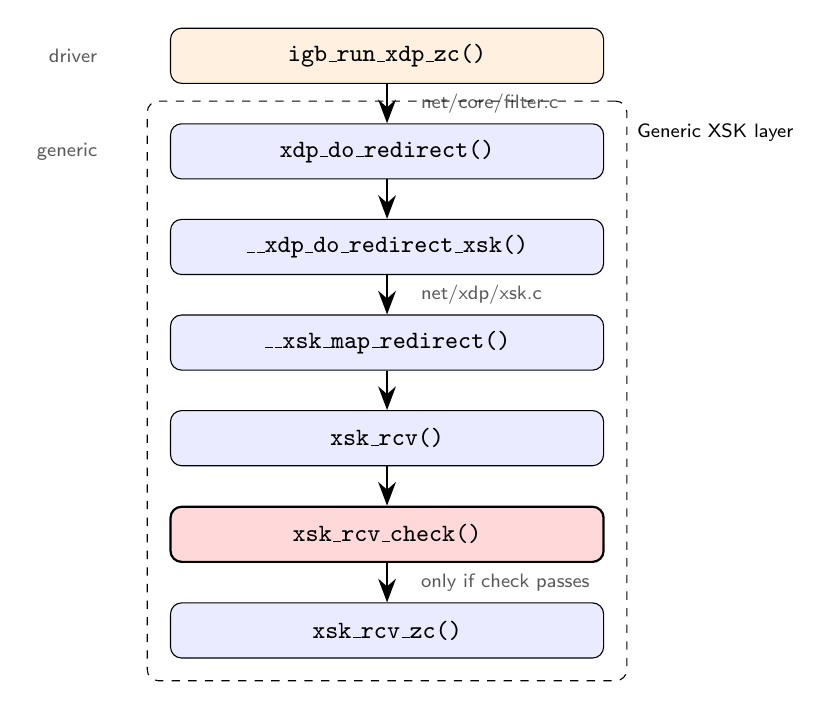
\begin{tikzpicture}[
    node distance=0.5cm,
    box/.style={draw, rounded corners, fill=blue!8, minimum width=5.5cm,
        minimum height=0.7cm, font=\ttfamily\small},
    driverbox/.style={draw, rounded corners, fill=orange!12, minimum width=5.5cm,
        minimum height=0.7cm, font=\ttfamily\small},
    guardbox/.style={draw, rounded corners, fill=red!15, minimum width=5.5cm,
        minimum height=0.7cm, font=\ttfamily\small, thick},
    arr/.style={-{Stealth[length=3mm]}, thick},
    lbl/.style={font=\scriptsize\sffamily, text=gray!70!black},
]
    \node[driverbox] (drv) {igb\_run\_xdp\_zc()};
    \node[box, below=of drv] (redir) {xdp\_do\_redirect()};
    \node[box, below=of redir] (xsk) {\_\_xdp\_do\_redirect\_xsk()};
    \node[box, below=of xsk] (map) {\_\_xsk\_map\_redirect()};
    \node[box, below=of map] (rcv) {xsk\_rcv()};
    \node[guardbox, below=of rcv] (chk) {xsk\_rcv\_check()};
    \node[box, below=of chk] (zc) {xsk\_rcv\_zc()};

    \draw[arr] (drv) -- (redir) node[lbl, midway, right, xshift=3mm]
        {net/core/filter.c};
    \draw[arr] (redir) -- (xsk);
    \draw[arr] (xsk) -- (map) node[lbl, midway, right, xshift=3mm]
        {net/xdp/xsk.c};
    \draw[arr] (map) -- (rcv);
    \draw[arr] (rcv) -- (chk);
    \draw[arr] (chk) -- (zc) node[lbl, midway, right, xshift=3mm]
        {only if check passes};

    \node[lbl, left=0.8cm of drv] {driver};
    \node[lbl, left=0.8cm of redir] {generic};

    \node[draw, dashed, rounded corners, fit=(redir)(xsk)(map)(rcv)(chk)(zc),
        inner sep=8pt, label={[font=\scriptsize\sffamily]above right:Generic XSK layer}] {};
\end{tikzpicture}
\caption{Call chain from driver NAPI handler to the queue\_id guard.
    The driver (orange) only calls \texttt{xdp\_do\_redirect()}; all
    subsequent logic is in generic kernel code. The guard (red) is the
    sole point of failure for cross-queue redirect.}
\label{fig:callchain}
\end{figure}

\subsection{Error Propagation and Silent Failure}

When \texttt{xsk\_rcv\_check()} returns \texttt{-EINVAL}, the error
propagates back up the call chain. The only visibility is a tracepoint
(\texttt{xdp:xdp\_redirect\_map\_err})---not a \texttt{pr\_warn} or
kernel log message. Unless the operator has \texttt{perf} attached to
that tracepoint, the failure is completely invisible.

Back in the driver, \texttt{igb\_run\_xdp\_zc()} checks the return value:

\begin{lstlisting}[caption={Error handling in igb\_run\_xdp\_zc().},
    label=lst:errhndl]
err = xdp_do_redirect(adapter->netdev, xdp, xdp_prog);
if (!err)
    return IGB_XDP_REDIR;

if (xsk_uses_need_wakeup(xsk_pool) && err == -ENOBUFS)
    result = IGB_XDP_EXIT;
else
    result = IGB_XDP_CONSUMED;
goto out_failure;
\end{lstlisting}

The redirect failure returns \texttt{IGB\_XDP\_CONSUMED}. The caller
(\texttt{igb\_clean\_rx\_irq\_zc()}) then calls \texttt{xsk\_buff\_free(xdp)}
to reclaim the buffer. The frame is properly freed---but from the BPF
program's perspective, \texttt{bpf\_redirect\_map} already returned
\texttt{XDP\_REDIRECT}, so the BPF-side counter incremented. This
creates a discrepancy between BPF counters (which show success) and
actual delivery (which failed).

\subsection{Documentation History}

The AF\_XDP maintainer Magnus Karlsson (Intel) briefly documented cross-queue
redirect as working with shared UMEM in kernel 6.9 (commit
\texttt{968595a93669}, February 2024), adding to
\texttt{Documentation/networking/af\_xdp.rst}:

\begin{quote}
\itshape
``it is also possible to redirect to any socket as long as it is bound to
the same umem with XDP\_SHARED\_UMEM''
\end{quote}

This was \textbf{reverted} in kernel 6.10 (commit \texttt{03e38d315f3c},
June 2024) after Yuval El-Hanany (Radware) reported that the documented
behavior was inaccurate---\texttt{xsk\_rcv\_check()} still enforced the
queue\_id match. The documentation was aspirational, describing what the
architecture supports rather than what the code permits.

The current kernel documentation explicitly states the limitation\\
(\texttt{Documentation/bpf/map\_xskmap.rst}):

\begin{quote}
\itshape
``An AF\_XDP socket that is bound to a certain $\langle$netdev/queue\_id$\rangle$
will \textbf{only} accept XDP frames from that
$\langle$netdev/queue\_id$\rangle$.''
\end{quote}

\section{Analysis: Why Cross-Queue Redirect Is Safe}

This section traces every stage of the redirect path and demonstrates that
cross-queue delivery is correct for aligned shared-UMEM configurations
without any driver modifications.

\subsection{Driver Ring Index Management}

The core of the safety argument rests on how the \texttt{igb} driver
(representative of all ZC-capable drivers) manages buffer ownership through
ring indices rather than per-slot state.

\begin{figure}[H]
\centering
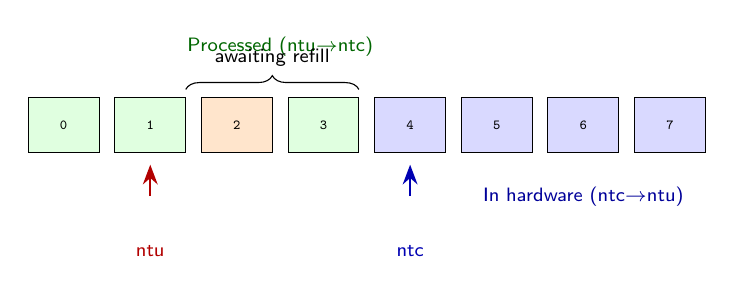
\begin{tikzpicture}[
    slot/.style={draw, minimum width=0.9cm, minimum height=0.7cm,
        font=\ttfamily\tiny},
    used/.style={slot, fill=blue!15},
    free/.style={slot, fill=green!12},
    redir/.style={slot, fill=orange!20},
    arr/.style={-{Stealth[length=2.5mm]}, thick},
]
    % Ring slots
    \foreach \i in {0,...,7} {
        \node[used] (s\i) at (\i*1.1, 0) {\i};
    }

    % Highlight zones
    \node[free, fill=green!12] at (0*1.1, 0) {0};
    \node[free, fill=green!12] at (1*1.1, 0) {1};
    \node[redir] at (2*1.1, 0) {2};
    \node[free, fill=green!12] at (3*1.1, 0) {3};

    % Labels
    \draw[arr, blue!70!black] (4*1.1, -0.9) -- (4*1.1, -0.5)
        node[below, yshift=-0.9cm, font=\scriptsize\sffamily] {ntc};
    \draw[arr, red!70!black] (1*1.1, -0.9) -- (1*1.1, -0.5)
        node[below, yshift=-0.9cm, font=\scriptsize\sffamily] {ntu};

    % Zone labels
    \node[font=\scriptsize\sffamily, text=blue!60!black] at (6*1.1, -0.9)
        {In hardware (ntc$\to$ntu)};
    \node[font=\scriptsize\sffamily, text=green!40!black] at (2.5*1.1, 1.0)
        {Processed (ntu$\to$ntc)};

    \draw[decorate, decoration={brace, amplitude=5pt, raise=3pt}]
        (1*1.1+0.45, 0.35) -- (3*1.1+0.45, 0.35)
        node[midway, above, yshift=8pt, font=\scriptsize\sffamily]
        {awaiting refill};
\end{tikzpicture}
\caption{RX descriptor ring after processing a redirect at slot 2.
    The redirected slot (orange) is in the ``processed'' zone between
    \texttt{ntu} and \texttt{ntc}. It will be overwritten with a fresh
    buffer on the next refill cycle.}
\label{fig:ring}
\end{figure}

In \texttt{igb\_clean\_rx\_irq\_zc()}, when the XDP result is
\texttt{IGB\_XDP\_REDIR}:

\begin{enumerate}[nosep]
    \item The driver does \textbf{not} call \texttt{xsk\_buff\_free(xdp)}---ownership
          has transferred to the generic redirect layer.
    \item \texttt{ntc} (next-to-clean) advances past the slot.
    \item The stale pointer in \texttt{rx\_buffer\_info\_zc[slot]} is now in the
          ``processed, awaiting refill'' zone.
    \item On refill, \texttt{igb\_alloc\_rx\_buffers\_zc()} calls
          \texttt{xsk\_buff\_alloc\_batch()} which writes a \textbf{new}
          \texttt{xdp\_buff} pointer into the slot, overwriting the stale one.
\end{enumerate}

This is identical to the same-queue redirect path. The driver cannot
distinguish between same-queue and cross-queue redirect---it calls
\texttt{xdp\_do\_redirect()} and acts on the return value. The target
queue is invisible to the driver.

\subsection{Buffer Lifecycle in \texttt{xsk\_rcv\_zc()}}

When a frame is successfully delivered (hypothetically, with the guard
removed), the generic layer executes:

\begin{lstlisting}[caption={Zero-copy receive path in \_\_xsk\_rcv\_zc().},
    label=lst:rcvzc]
static int __xsk_rcv_zc(struct xdp_sock *xs,
        struct xdp_buff_xsk *xskb, u32 len, u32 flags)
{
    u64 addr;
    int err;

    addr = xp_get_handle(xskb, xskb->pool);
    err = xskq_prod_reserve_desc(xs->rx, addr, len, flags);
    if (err) {
        xs->rx_queue_full++;
        return err;
    }

    xp_release(xskb);
    return 0;
}
\end{lstlisting}

Three operations occur:

\begin{enumerate}[nosep]
    \item \texttt{xp\_get\_handle()} computes the UMEM offset from the
          \texttt{xdp\_buff\_xsk}. With shared UMEM, the offset is valid
          regardless of which queue's pool allocated the buffer---it's all
          the same mmap'd region.

    \item \texttt{xskq\_prod\_reserve\_desc()} writes the descriptor (UMEM
          address + length) to the target socket's RX ring. This is a simple
          ring buffer append with no queue affinity.

    \item \texttt{xp\_release()} for aligned pools is a \textbf{no-op}:
\end{enumerate}

\begin{lstlisting}[caption={xp\_release() is a no-op for aligned pools.},
    label=lst:release]
static inline void xp_release(struct xdp_buff_xsk *xskb)
{
    if (xskb->pool->unaligned)
        xskb->pool->free_heads[
            xskb->pool->free_heads_cnt++] = xskb;
    /* aligned mode: nothing to do */
}
\end{lstlisting}

For aligned pools (the common case, including any configuration using
the default 4096-byte chunk size), \texttt{xdp\_buff\_xsk} structures
are statically indexed by \texttt{addr / chunk\_size} in the pool's
\texttt{heads[]} array. They are not dynamically allocated or freed---they
are looked up fresh from the fill queue address each time
\texttt{xp\_get\_xskb()} is called during buffer allocation.

\subsection{Teardown Safety}

A concern was raised that ring teardown could double-free redirected
buffers. The teardown function \texttt{igb\_clean\_rx\_ring\_zc()} iterates
only from \texttt{ntc} to \texttt{ntu}---the range of buffers currently
posted to hardware and not yet processed:

\begin{lstlisting}[caption={Ring teardown only frees unprocessed buffers.},
    label=lst:teardown]
void igb_clean_rx_ring_zc(struct igb_ring *rx_ring)
{
    u16 ntc = rx_ring->next_to_clean;
    u16 ntu = rx_ring->next_to_use;

    while (ntc != ntu) {
        struct xdp_buff *xdp =
            rx_ring->rx_buffer_info_zc[ntc];
        xsk_buff_free(xdp);
        ntc++;
        if (ntc >= rx_ring->count)
            ntc = 0;
    }
}
\end{lstlisting}

A redirected buffer has already been processed (\texttt{ntc} advanced
past its slot in \texttt{igb\_clean\_rx\_irq\_zc()}).
It is therefore outside the \texttt{ntc}$\to$\texttt{ntu} range and
will not be freed. Furthermore, teardown cannot race with NAPI because
\texttt{igb\_txrx\_ring\_disable()} calls
\texttt{napi\_disable()} before touching ring state, ensuring
\texttt{ntc} reflects all completed processing.

\subsection{DMA Coherency}

With shared UMEM, DMA mappings are established at the pool level via
\texttt{xsk\_pool\_dma\_map()}, not per-buffer. Each queue's pool maps
the same UMEM pages to the same device, producing identical DMA addresses
for the same UMEM offsets. The per-buffer CPU cache sync
(\texttt{xsk\_buff\_dma\_sync\_for\_cpu()}) is performed on the source
queue before the XDP program executes---before any redirect decision.
No additional sync is needed for cross-queue delivery, as userspace on
the target queue simply reads from CPU-coherent memory.

\subsection{Error Handling}

The driver correctly handles redirect failures. As shown in
Listing~\ref{lst:errhndl}, \texttt{igb\_run\_xdp\_zc()} checks
\texttt{xdp\_do\_redirect()}'s return value. On failure (e.g., target RX
ring full), the buffer is freed via \texttt{xsk\_buff\_free()} in the
\texttt{IGB\_XDP\_CONSUMED} path. No buffer leaks occur on redirect failure,
whether same-queue or cross-queue.

\section{Counterarguments Considered}

Several potential objections to relaxing the guard were raised during
analysis. We address each in turn.

\subsection{Fill Ring Depletion}

\textbf{Concern:} If frames consistently migrate from queue $X$ to queue $Y$
via cross-queue redirect, queue $X$'s fill ring drains over time (frames
allocated from $X$'s fill ring are consumed by $Y$'s RX ring and returned
to $Y$'s fill ring by userspace).

\medskip\noindent
\textbf{Response:} This is an application-level resource management
concern, not a kernel invariant violation. With shared UMEM, all UMEM
addresses are valid on any queue's fill ring. A well-designed application
maintains a global free pool of frame descriptors and redistributes them
across fill rings based on demand. Applications that use
\texttt{XDP\_SHARED\_UMEM} are already managing multi-queue buffer
lifecycle; cross-queue frame migration is a natural extension.

The kernel does not prevent userspace from submitting ``foreign'' UMEM
addresses to any fill ring today. The fill ring consumer
(\texttt{xp\_alloc\_new\_from\_fq()}) accepts any valid UMEM offset.

\subsection{Unaligned Mode Pool Leaking}

\textbf{Concern:} For unaligned pools (\texttt{XDP\_UMEM\_UNALIGNED\_CHUNK\_FLAG}),
\texttt{xp\_release()} adds the \texttt{xdp\_buff\_xsk} back to
\texttt{pool->free\_heads[]}. Cross-queue redirect would return xskb
entries to the source pool's free list, while the target pool's
\texttt{free\_heads\_cnt} would shrink over time.

\medskip\noindent
\textbf{Response:} This is a valid concern for unaligned mode and would
need to be addressed separately. However, aligned mode (the default and
overwhelmingly common configuration) is unaffected because
\texttt{xp\_release()} is a no-op---\texttt{xdp\_buff\_xsk} structures
are statically indexed and never moved between free lists.

A proposed patch could initially restrict cross-queue redirect to aligned
pools and address unaligned mode in a follow-up.

\subsection{Driver-Specific Complications}

\textbf{Concern:} Drivers maintain hidden per-queue state beyond the ring
indices, and cross-queue redirect could corrupt this state.

\medskip\noindent
\textbf{Response:} In ZC mode, the driver's per-buffer state is exactly
one pointer:\\
\texttt{rx\_buffer\_info\_zc[slot]}.
There is no per-buffer
DMA mapping, no page reference, no metadata structure. The pointer is
overwritten on refill with a fresh allocation. The driver has no
``hidden accounting'' beyond the ring indices.

This was verified for \texttt{igb} and holds for all upstream ZC drivers
(\texttt{ice}, \texttt{igc}, \texttt{i40e}, \texttt{mlx5}), which follow
the same pattern: read \texttt{xdp\_buff} from slot, run XDP, advance
index on redirect, refill with new allocation.

Critically, the driver never learns the target queue of a redirect. It
calls \texttt{xdp\_do\_redirect()} and gets back success or failure.
The generic XSK layer handles all target-queue logic. Cross-queue redirect
requires zero changes to any driver.

\subsection{The \texttt{bpf\_redirect\_map} API Confusion}

\textbf{Concern:} Why does \texttt{bpf\_redirect\_map(\&xsks\_map, key, 0)}
accept a key that can differ from \texttt{ctx->rx\_queue\_index} if
cross-queue delivery doesn't work?

\medskip\noindent
\textbf{Response:} \texttt{bpf\_redirect\_map} is a generic helper shared
across three map types (Table~\ref{tab:maptypes}). For \texttt{DEVMAP} and
\texttt{CPUMAP}, cross-target redirect is the entire purpose. For
\texttt{XSKMAP}, the key is a map lookup index that happens to conventionally
equal the queue index. The BPF verifier cannot distinguish the map type
at verification time, so it accepts any key. The API ambiguity is an
artifact of generality, not a feature.

\begin{table}[H]
\centering
\caption{Behavior of \texttt{bpf\_redirect\_map} across map types.}
\label{tab:maptypes}
\begin{tabular}{lll}
\toprule
\textbf{Map type} & \textbf{Index meaning} & \textbf{Cross-target?} \\
\midrule
\texttt{BPF\_MAP\_TYPE\_DEVMAP} & target netdev & Yes \\
\texttt{BPF\_MAP\_TYPE\_CPUMAP} & target CPU & Yes \\
\texttt{BPF\_MAP\_TYPE\_XSKMAP} & socket map key & \textbf{No} (guard) \\
\bottomrule
\end{tabular}
\end{table}

\section{Proposed Kernel Patch}

\subsection{Approach}

Relax the \texttt{queue\_id} check in \texttt{xsk\_rcv\_check()} to allow
cross-queue redirect when the source and target sockets share the same
UMEM and the pool uses aligned chunks. The check remains in place for:

\begin{itemize}[nosep]
    \item Cross-device redirect (different \texttt{netdev})---remains blocked.
    \item Non-shared-UMEM sockets---remains blocked.
    \item Unaligned mode---remains blocked (pending separate analysis).
\end{itemize}

\subsection{Proposed Diff}

The removed lines are shown in \colorbox{red!12}{red} and added lines in
\colorbox{green!12}{green}:

\begin{lstlisting}[caption={Proposed change to xsk\_rcv\_check().},
    label=lst:patch, numbers=none]
 static int xsk_rcv_check(struct xdp_sock *xs,
                          struct xdp_buff *xdp, u32 len)
 {
     if (!xsk_is_bound(xs))
         return -ENXIO;
\end{lstlisting}
\vspace{-1.2em}
\begin{lstlisting}[numbers=none, backgroundcolor=\color{red!12}]
-    if (xs->dev != xdp->rxq->dev ||
-        xs->queue_id != xdp->rxq->queue_index)
\end{lstlisting}
\vspace{-1.2em}
\begin{lstlisting}[numbers=none, backgroundcolor=\color{green!12}]
+    if (xs->dev != xdp->rxq->dev)
+        return -EINVAL;
+
+    if (xs->queue_id != xdp->rxq->queue_index &&
+        !xsk_pool_same_umem(xs->pool, xdp))
\end{lstlisting}
\vspace{-1.2em}
\begin{lstlisting}[numbers=none]
         return -EINVAL;

     if (len > xsk_pool_get_rx_frame_size(xs->pool)
         && !xs->sg) {
         xs->rx_dropped++;
         return -ENOSPC;
     }

     return 0;
 }
\end{lstlisting}

Where \texttt{xsk\_pool\_same\_umem()} is a new helper:

\begin{lstlisting}[caption={Helper to check shared UMEM between source and target.},
    label=lst:helper]
static inline bool xsk_pool_same_umem(
    struct xsk_buff_pool *target_pool,
    struct xdp_buff *xdp)
{
    struct xsk_buff_pool *src_pool;

    src_pool = xdp->rxq->dev->_rx[
        xdp->rxq->queue_index].pool;
    if (!src_pool || !target_pool)
        return false;

    return target_pool->umem == src_pool->umem
        && !target_pool->unaligned;
}
\end{lstlisting}

\subsection{What This Enables}

With this change, an XDP program can redirect a packet arriving on any
hardware queue to any AF\_XDP socket on the same device, provided all
sockets share the same UMEM via \texttt{XDP\_SHARED\_UMEM} with aligned
chunks. The application receives the frame on the target socket's RX ring
and is responsible for returning the UMEM frame descriptor to an
appropriate fill ring.

\subsection{What This Does Not Change}

\begin{itemize}[nosep]
    \item No driver code is modified.
    \item No new BPF helpers or map types are introduced.
    \item The existing \texttt{bpf\_redirect\_map} API is used as-is.
    \item Cross-device redirect remains blocked.
    \item Unaligned UMEM remains blocked (future work).
    \item Applications that do not use cross-queue redirect are unaffected.
\end{itemize}

\section{Testing Strategy}

A patch submission should include:

\begin{enumerate}[nosep]
    \item \textbf{Selftest extension:} Extend\\
          \texttt{tools/testing/selftests/bpf/prog\_tests/xdp\_do\_redirect.c}\\
          with a cross-queue shared-UMEM test case.
    \item \textbf{xsk selftest:} Extend
          \texttt{tools/testing/selftests/bpf/xskxceiver.c} with
          cross-queue redirect scenarios (same device, shared UMEM,
          aligned chunks).
    \item \textbf{Negative tests:} Verify that cross-queue redirect still
          fails for non-shared UMEM and unaligned mode.
    \item \textbf{Stress testing:} Sustained cross-queue traffic to verify
          no fill ring depletion, buffer leaks, or pool corruption under
          load. The application must actively redistribute frame descriptors.
    \item \textbf{Multi-driver validation:} Test on at least \texttt{igb},
          \texttt{igc}, and \texttt{ice} to confirm no driver-specific
          regressions.
\end{enumerate}

\section{Conclusion}

The \texttt{queue\_id} guard in \texttt{xsk\_rcv\_check()} is the sole
barrier to cross-queue XDP redirect with AF\_XDP shared UMEM in zero-copy
mode. Tracing the complete code path from driver NAPI handler through
generic XSK infrastructure demonstrates that:

\begin{itemize}[nosep]
    \item Driver ring management correctly handles buffer ownership transfer
          for redirected frames (same mechanism as same-queue redirect).
    \item No driver modifications are required---the driver is unaware of
          the redirect target.
    \item DMA coherency is maintained at the UMEM/pool level.
    \item Teardown and error paths are safe.
    \item For aligned pools, \texttt{xdp\_buff\_xsk} accounting is
          statically indexed and cannot leak across pools.
\end{itemize}

The guard was appropriate as a conservative default when AF\_XDP was
introduced, and it remains correct for non-shared-UMEM and unaligned
configurations. However, for the aligned shared-UMEM case---which
represents the majority of multi-queue AF\_XDP deployments---the
restriction prevents a natural and architecturally sound use of XDP
redirect for intra-application packet steering.

We propose a minimal, targeted relaxation: allow cross-queue redirect
when the source and target sockets demonstrably share the same UMEM
with aligned chunks. This change is confined to a single function in
generic XSK code, requires no driver modifications, and is gated
behind conditions that ensure buffer accounting integrity.

\end{document}
